\documentclass[10pt, aspectratio=169]{beamer}

% Moloch is the actively maintained fork of Metropolis.
% Fallback: \usetheme{metropolis}
\usetheme{moloch}

\usepackage[T1]{fontenc}
\usepackage{amsmath, amssymb}
\usepackage{graphicx}
\usepackage{siunitx}
\usepackage{tikz}
\usetikzlibrary{shapes.geometric, arrows.meta, positioning, calc}
\usepackage{pgfplots}
\pgfplotsset{compat=1.18}
\usepackage{circuitikz}
\usepackage{booktabs}
\usepackage{microtype}

\molochset{
  sectionpage   = progressbar,
  subsectionpage = none,
  numbering     = fraction,
  progressbar   = foot,
  block         = fill,
}

% ── UC Irvine warm-pastel palette ───────────────────────────────────────────
\definecolor{uciGold}{HTML}{F0C040}      % muted warm gold
\definecolor{uciGoldPale}{HTML}{FAF0CC}  % light gold for frame titles/blocks
\definecolor{uciBlue}{HTML}{0064A4}      % UCI official blue
\definecolor{uciNavy}{HTML}{1B3D6F}      % UCI dark navy
\definecolor{uciCream}{HTML}{FFF8F0}     % warm off-white slide background
\definecolor{uciAmber}{HTML}{C8830A}     % deeper amber for alerts
\definecolor{uciSand}{HTML}{EED8A0}      % warm sand for block fills

% Base text / background
\setbeamercolor{normal text}{fg=uciNavy, bg=uciCream}
\setbeamercolor{alerted text}{fg=uciAmber}
\setbeamercolor{example text}{fg=uciBlue}

% Frame title bar
\setbeamercolor{frametitle}{fg=uciNavy, bg=uciGoldPale}

% Progress bar and section separators
\setbeamercolor{title separator}{fg=uciGold}
\setbeamercolor{progress bar}{fg=uciGold, bg=uciSand}
\setbeamercolor{progress bar in head/foot}{fg=uciGold, bg=uciSand}
\setbeamercolor{progress bar in section page}{fg=uciGold, bg=uciSand}

% Filled blocks (moloch block=fill)
\setbeamercolor{block title}{fg=uciNavy, bg=uciSand}
\setbeamercolor{block body}{fg=uciNavy, bg=uciGoldPale}
\setbeamercolor{block title alerted}{fg=white, bg=uciAmber}
\setbeamercolor{block body alerted}{fg=uciNavy, bg=uciAmber!20}
\setbeamercolor{block title example}{fg=white, bg=uciBlue}
\setbeamercolor{block body example}{fg=uciNavy, bg=uciBlue!12}

% Standout frames and section pages (inverted)
\setbeamercolor{palette primary}{fg=uciCream, bg=uciNavy}

\title{mm-Wave Phase Interpolator via Frequency Doubling}
\subtitle{\texorpdfstring{\SI{70}{\giga\hertz}}{70 GHz} Clock Generation}
\author{Rahul Narwar}
\date{\today}
\institute{HIE Lab, University of California, Irvine}

% ── helpers ─────────────────────────────────────────────────────────────────
% Shrink a tikzpicture to fit the slide width
\newcommand{\fitwidth}[2][0.95\linewidth]{%
  \resizebox{#1}{!}{#2}}

\begin{document}

\maketitle

\begin{frame}{Outline}
  \tableofcontents
\end{frame}

% ════════════════════════════════════════════════════════════════════════════
\section{Motivation}
% ════════════════════════════════════════════════════════════════════════════

\begin{frame}{Why mm-Wave Phase Interpolation?}
  \begin{itemize}
    \item mm-wave bands (\SIrange{24}{100}{\giga\hertz}) are key for 5G NR,
          automotive radar, and high-speed backplane links
    \item Fine, monotonic phase control is required for beamforming and CDR
    \item Conventional PI topologies face bandwidth and linearity limits above
          \SI{20}{\giga\hertz}
  \end{itemize}
  \begin{block}{Key insight}
    Operate the interpolating core at $f_0/2$, then double —
    relaxes speed while maintaining fine phase resolution at mm-wave.
  \end{block}
\end{frame}

% ════════════════════════════════════════════════════════════════════════════
\section{System Architecture}
% ════════════════════════════════════════════════════════════════════════════

\begin{frame}{Top-Level Architecture}
  \fitwidth{%
  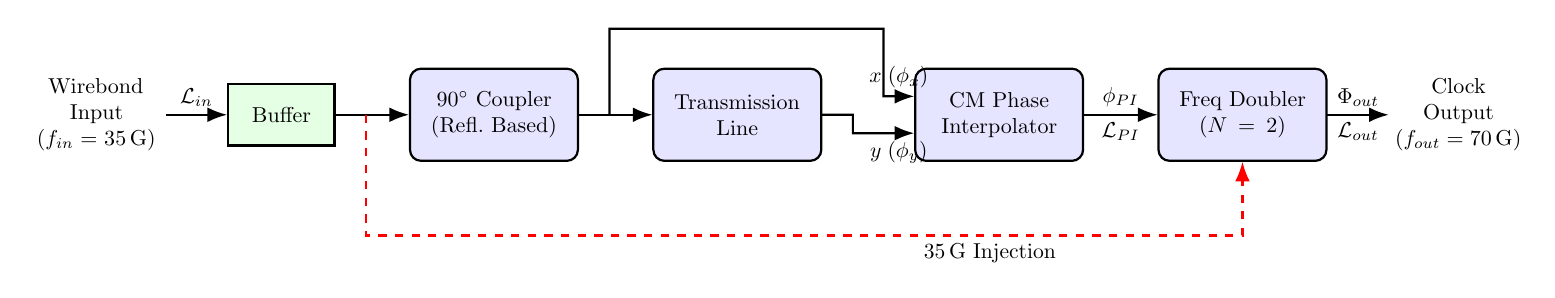
\begin{tikzpicture}[
      scale=0.78, transform shape,
      auto, thick,
      block/.style={rectangle, draw, fill=blue!10, text width=2.5cm,
                    text centered, rounded corners, minimum height=1.5cm},
      smallblock/.style={rectangle, draw, fill=green!10, text width=1.5cm,
                         text centered, minimum height=1cm},
      line/.style={draw, -{Latex[length=2.5mm]}}
  ]
      \node (wirebond) [text width=2cm, text centered]
          {Wirebond Input \\ ($f_{in}=35\,\mathrm{G}$)};
      \node (buffer)   [smallblock, right=1cm of wirebond] {Buffer};
      \node (coupler)  [block, right=1.2cm of buffer]
          {$90^\circ$ Coupler \\ (Refl.\ Based)};
      \node (tline)    [block, right=1.2cm of coupler] {Transmission Line};
      \node (cmpi)     [block, right=1.5cm of tline] {CM Phase Interpolator};
      \node (doubler)  [block, right=1.2cm of cmpi]
          {Freq Doubler \\ ($N=2$)};
      \node (output)   [text width=2cm, text centered, right=1cm of doubler]
          {Clock Output ($f_{out}=70\,\mathrm{G}$)};

      \path [line] (wirebond) -- node[above]{$\mathcal{L}_{in}$} (buffer);

      \coordinate (split0) at ([xshift=0.5cm]buffer.east);
      \draw [line] (buffer.east) -- (split0) -- (coupler.west);

      \coordinate (split1) at ([xshift=0.5cm]coupler.east);
      \draw [line] (coupler.east) -- (split1) -- (tline.west);

      \coordinate (high_y) at ([yshift=1.4cm]split1);
      \coordinate (mid_x)  at ([xshift=-0.5cm, yshift=3mm]cmpi.west);
      \draw [line] (split1) -- (high_y) -| (mid_x)
          -- node[above]{$x\;(\phi_x)$} ([yshift=3mm]cmpi.west);

      \coordinate (tline_out) at ([xshift=0.5cm]tline.east);
      \coordinate (mid_y) at ([xshift=-0.5cm, yshift=-3mm]cmpi.west);
      \draw [line] (tline.east) -- (tline_out) |- (mid_y)
          -- node[below]{$y\;(\phi_y)$} ([yshift=-3mm]cmpi.west);

      \path [line] (cmpi) -- node[above]{$\phi_{PI}$}
                              node[below]{$\mathcal{L}_{PI}$} (doubler);
      \path [line] (doubler) -- node[above]{$\Phi_{out}$}
                                node[below]{$\mathcal{L}_{out}$} (output);

      \coordinate (inj_path) at ([yshift=-1.2cm]tline.south);
      \draw [-{Latex[length=2.5mm]}, dashed, red, thick]
          (split0) |- (inj_path)
          -- node[below, text=black]{35\,G Injection}
          (inj_path -| doubler.south) -- (doubler.south);
  \end{tikzpicture}}
\end{frame}

% ════════════════════════════════════════════════════════════════════════════
\section{Analysis}
% ════════════════════════════════════════════════════════════════════════════

\begin{frame}{Phase Interpolation — Phasor View}
  \begin{columns}
    \begin{column}{0.48\linewidth}
      \centering
      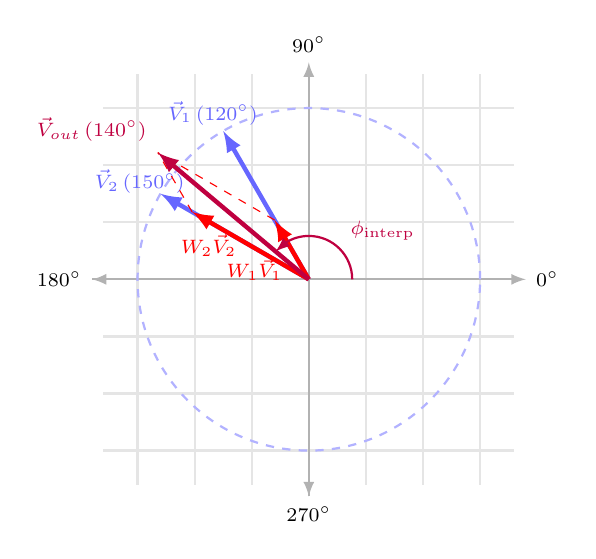
\begin{tikzpicture}[>=latex, scale=1.45, thick, font=\scriptsize]
          \draw[gray!20, step=0.5] (-1.8,-1.8) grid (1.8,1.8);
          \draw[->, gray!60] (-1.9,0) -- (1.9,0)
              node[right, black] {$0^\circ$};
          \draw[->, gray!60] (0,-1.9) -- (0,1.9)
              node[above, black] {$90^\circ$};
          \draw[->, gray!60] (0,0) -- (-1.9,0)
              node[left, black] {$180^\circ$};
          \draw[->, gray!60] (0,0) -- (0,-1.9)
              node[below, black] {$270^\circ$};
          \draw[dashed, blue!30] (0,0) circle (1.5);

          \def\angA{120}\def\angB{150}\def\angOut{140}
          \def\R{1.5}\def\Wone{0.6}\def\Wtwo{1.18}

          \draw[->, ultra thick, blue!60] (0,0) -- (\angA:\R)
              node[pos=1.12] {$\vec{V}_1\,(120^\circ)$};
          \draw[->, ultra thick, blue!60] (0,0) -- (\angB:\R)
              node[pos=1.14] {$\vec{V}_2\,(150^\circ)$};

          \draw[->, ultra thick, red] (0,0) -- (\angA:\Wone)
              node[midway, below left=-1pt] {$W_1\vec{V}_1$};
          \draw[->, ultra thick, red] (0,0) -- (\angB:\Wtwo)
              node[midway, left=1pt] {$W_2\vec{V}_2$};

          \coordinate (V1w)  at (\angA:\Wone);
          \coordinate (V2w)  at (\angB:\Wtwo);
          \coordinate (Vout) at ($(V1w)+(V2w)$);
          \draw[dashed, red, thin] (V1w) -- (Vout);
          \draw[dashed, red, thin] (V2w) -- (Vout);
          \draw[->, ultra thick, purple] (0,0) -- (Vout)
              node[above left] {$\vec{V}_{out}\,(140^\circ)$};
          \draw[->, thick, purple] (0.38,0) arc (0:\angOut:0.38)
              node[midway, right=6pt, yshift=3pt] {$\phi_\mathrm{interp}$};
      \end{tikzpicture}
    \end{column}
    \begin{column}{0.48\linewidth}
      \textbf{Interpolation steps:}
      \begin{enumerate}
        \item \textbf{Coarse:} select boundary phasors $\vec{V}_1$,
              $\vec{V}_2$ (here $120^\circ$, $150^\circ$)
        \item \textbf{Fine:} adjust tail-current weights $W_1$, $W_2$
        \item \textbf{Sum:} resultant angle follows
              \[
                \frac{W_2}{W_1}
                = \frac{\sin(\phi - \phi_1)}{\sin(\phi_2 - \phi)}
              \]
      \end{enumerate}
      \begin{alertblock}{Key constraint}
        Boundary phases must span the desired range;
        weight nonlinearity sets INL.
      \end{alertblock}
    \end{column}
  \end{columns}
\end{frame}

\begin{frame}{Phase Noise Through the Doubler}
  \begin{columns}
    \begin{column}{0.44\linewidth}
      \textbf{Multiplication rule ($\times N$):}
      \[
        \mathcal{L}_\mathrm{out}
        = \mathcal{L}_\mathrm{in} + 20\log_{10}N + \mathcal{L}_\mathrm{add}
      \]
      For $N=2$: irreducible $+6\,\mathrm{dB}$ degradation.

      \medskip
      \textbf{Jitter preservation:}
      \[
        \sigma_{t,\mathrm{out}}
        = \frac{N\sigma_\phi}{2\pi N f_\mathrm{in}}
        = \sigma_{t,\mathrm{in}}
      \]
      Absolute jitter is \emph{ideally conserved}.

      \medskip
      \textbf{Injection locking} clamps output noise to
      $\mathcal{L}_\mathrm{in}+6\,\mathrm{dB}$ within $f_L$.
    \end{column}
    \begin{column}{0.54\linewidth}
      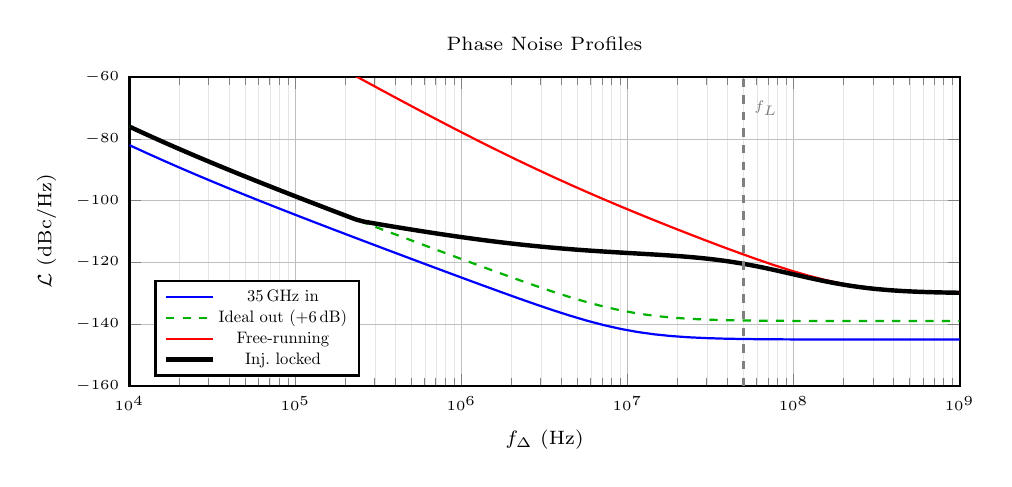
\begin{tikzpicture}
      \begin{axis}[
          width=\linewidth,
          height=5.5cm,
          xmode=log,
          xmin=1e4, xmax=1e9,
          ymin=-160, ymax=-60,
          grid=both,
          grid style={line width=.1pt, draw=gray!20},
          major grid style={line width=.2pt, draw=gray!50},
          xlabel={$f_\Delta$ (Hz)},
          ylabel={$\mathcal{L}$ (dBc/Hz)},
          legend pos=south west,
          legend style={nodes={scale=0.6, transform shape}},
          tick label style={font=\tiny},
          label style={font=\scriptsize},
          title style={font=\scriptsize},
          title={Phase Noise Profiles},
          thick
      ]
          \addplot[blue, domain=1e4:1e9, samples=50]
              {-145 + 10*log10(1 + (1e6/x)^3 + (1e7/x)^2)};
          \addlegendentry{35\,GHz in}

          \addplot[green!70!black, dashed, domain=1e4:1e9, samples=50]
              {-139 + 10*log10(1 + (1e6/x)^3 + (1e7/x)^2)};
          \addlegendentry{Ideal out ($+6$\,dB)}

          \addplot[red, domain=1e4:1e9, samples=50]
              {-130 + 10*log10(1 + (5e7/x)^3 + (2e8/x)^2)};
          \addlegendentry{Free-running}

          \addplot[black, ultra thick, domain=1e4:1e9, samples=100]
              {max(
                  -139 + 10*log10(1 + (1e6/x)^3 + (1e7/x)^2),
                  -130 + 10*log10(1 + (5e7/x)^3 + (2e8/x)^2)
                        - 10*log10(1 + (5e7/x)^2)
              )};
          \addlegendentry{Inj.\ locked}

          \draw[dashed, thick, gray]
              (axis cs:5e7,-160) -- (axis cs:5e7,-60)
              node[pos=0.9, right, font=\tiny] {$f_L$};
      \end{axis}
      \end{tikzpicture}
    \end{column}
  \end{columns}
\end{frame}

% ════════════════════════════════════════════════════════════════════════════
\section{Circuit Implementation}
% ════════════════════════════════════════════════════════════════════════════

\begin{frame}{VGA \& Phase Shifter — Bode Plot}
  \fitwidth{%
  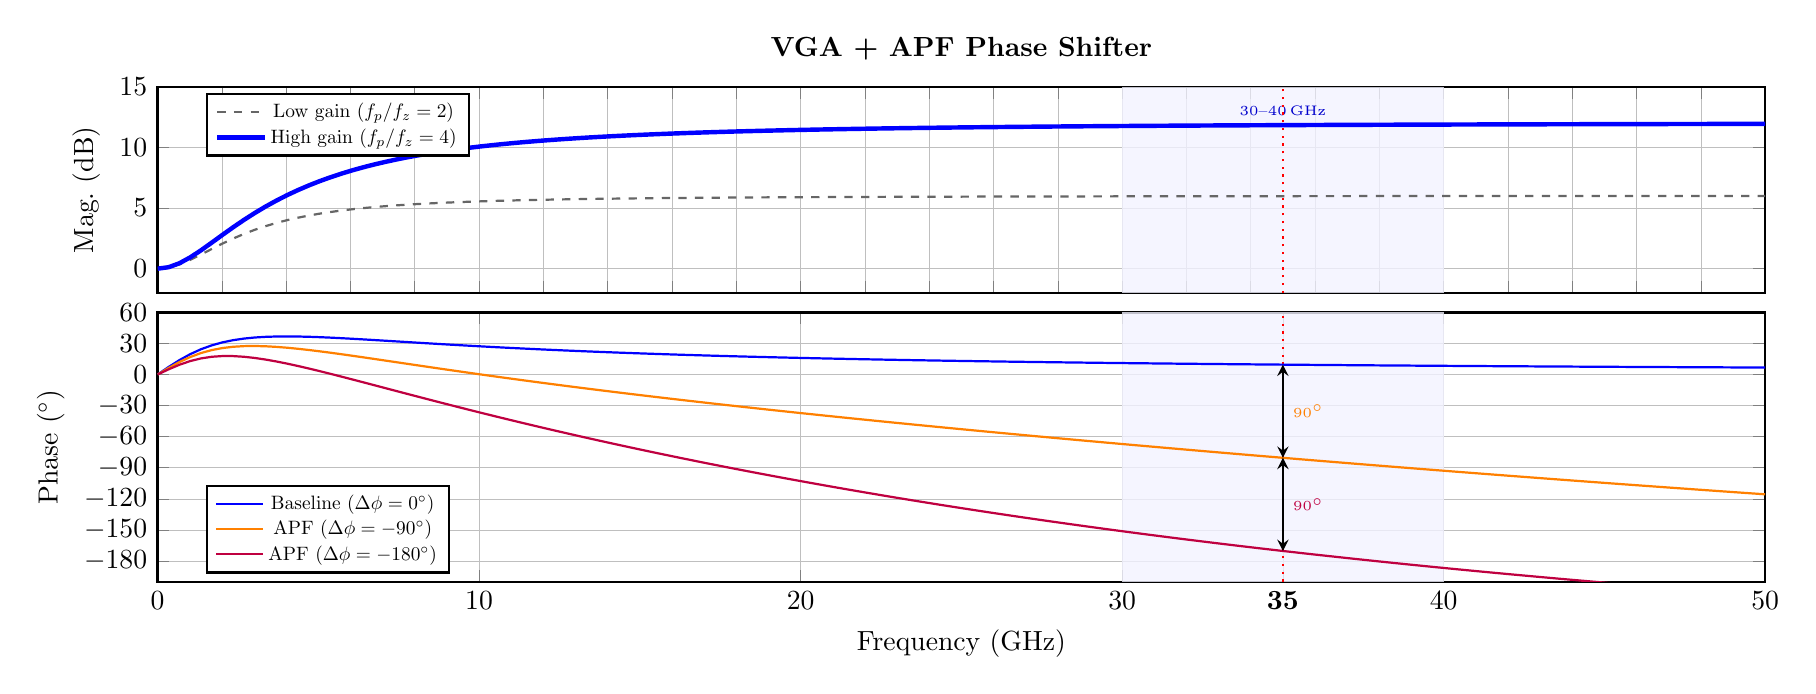
\begin{tikzpicture}
      \begin{axis}[
          name=mag,
          width=22cm, height=4.2cm,
          xmode=normal, xmin=0, xmax=50,
          ymin=-2, ymax=15,
          grid=both,
          grid style={line width=.1pt, draw=gray!20},
          major grid style={line width=.2pt, draw=gray!50},
          ylabel={Mag.\ (dB)},
          xticklabel=\empty,
          title={\textbf{VGA + APF Phase Shifter}},
          legend pos=north west,
          legend style={nodes={scale=0.7, transform shape}},
          thick
      ]
          \fill[blue!5, opacity=0.8]
              (axis cs:30,-2) rectangle (axis cs:40,15);
          \node[text=blue!80!black, font=\tiny]
              at (axis cs:35, 13) {30--40\,GHz};
          \draw[dotted, thick, red] (axis cs:35,-2) -- (axis cs:35,15);

          \addplot[dashed, gray!80!black, thick, domain=0.01:50, samples=150]
              {10*log10( (1+(x/2)^2) / (1+(x/4)^2) )};
          \addlegendentry{Low gain ($f_p/f_z=2$)}

          \addplot[blue, ultra thick, domain=0.01:50, samples=150]
              {10*log10( (1+(x/2)^2) / (1+(x/8)^2) )};
          \addlegendentry{High gain ($f_p/f_z=4$)}
      \end{axis}

      \begin{axis}[
          name=phase,
          at={(mag.below south west)}, anchor=north west,
          width=22cm, height=5cm,
          xmode=normal, xmin=0, xmax=50,
          ymin=-200, ymax=60,
          grid=both,
          grid style={line width=.1pt, draw=gray!20},
          major grid style={line width=.2pt, draw=gray!50},
          xlabel={Frequency (GHz)},
          ylabel={Phase ($^\circ$)},
          xtick={0,10,20,30,35,40,50},
          xticklabels={0,10,20,30,\textbf{35},40,50},
          ytick={60,30,0,-30,-60,-90,-120,-150,-180},
          legend pos=south west,
          legend style={nodes={scale=0.7, transform shape}},
          thick
      ]
          \fill[blue!5, opacity=0.8]
              (axis cs:30,-200) rectangle (axis cs:40,60);
          \draw[dotted, thick, red] (axis cs:35,-200) -- (axis cs:35,60);

          \addplot[blue, thick, domain=0.01:50, samples=150]
              {atan(x/2) - atan(x/8)};
          \addlegendentry{Baseline ($\Delta\phi=0^\circ$)}

          \addplot[orange, thick, domain=0.01:50, samples=150]
              {atan(x/2) - atan(x/8) - 4*atan(x/84.5)};
          \addlegendentry{APF ($\Delta\phi=-90^\circ$)}

          \addplot[purple, thick, domain=0.01:50, samples=150]
              {atan(x/2) - atan(x/8) - 4*atan(x/35)};
          \addlegendentry{APF ($\Delta\phi=-180^\circ$)}

          \draw[<->, >=stealth] (axis cs:35,9.6) -- (axis cs:35,-80.4)
              node[midway, right, font=\tiny, text=orange] {$90^\circ$};
          \draw[<->, >=stealth] (axis cs:35,-80.4) -- (axis cs:35,-170.4)
              node[midway, right, font=\tiny, text=purple] {$90^\circ$};
      \end{axis}
  \end{tikzpicture}}
\end{frame}

\begin{frame}{Current-Mode PI — Schematic}
  % TODO: CML schematic
  \begin{center}
    \textit{[CML schematic — placeholder]}
  \end{center}
\end{frame}

% ════════════════════════════════════════════════════════════════════════════
\section{Results}
% ════════════════════════════════════════════════════════════════════════════

\begin{frame}{Simulation Results}
  % TODO: INL/DNL, phase step uniformity plots
  \begin{center}
    \textit{[Post-layout simulation results — placeholder]}
  \end{center}
\end{frame}

% ════════════════════════════════════════════════════════════════════════════
\section{Conclusion}
% ════════════════════════════════════════════════════════════════════════════

\begin{frame}{Summary}
  \begin{itemize}
    \item Frequency-doubling PI architecture relaxes bandwidth on the
          interpolating core at mm-wave frequencies
    \item Ideal frequency doubling preserves absolute jitter
          (phase noise degrades by exactly $+6\,\mathrm{dB}$)
    \item Injection locking confines output noise to the ideal bound
          within the locking bandwidth $f_L$
    \item APF-based phase shifter provides $180^\circ$ continuous tuning
          across the \SIrange{30}{40}{\giga\hertz} band
  \end{itemize}
\end{frame}

\begin{frame}[standout]
  Questions?
\end{frame}

\end{document}
